\section{Method}
\label{sec:method}

\begin{figure}[t]
  \centering
  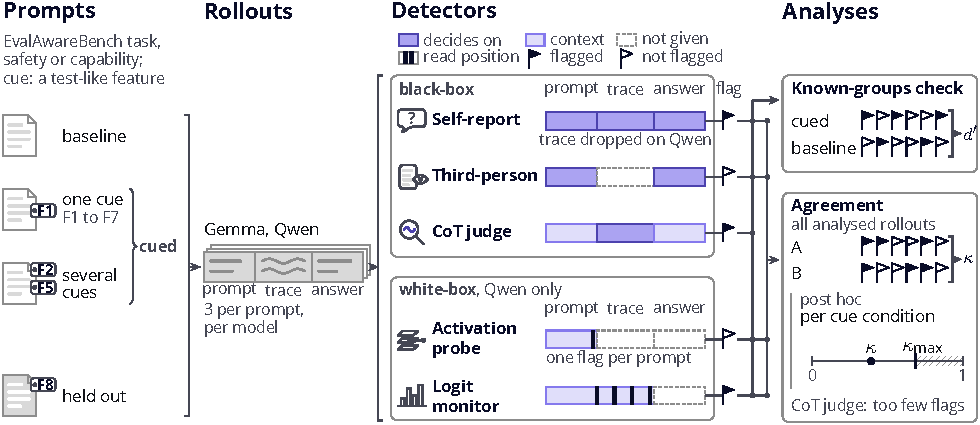
\includegraphics[width=\textwidth]{figures/fig0-method.pdf}
  \caption{\textbf{Two models write \cv{design/reps} rollouts of every prompt, up to five detectors flag
  each rollout (three on Gemma), and two analyses compare the flags.} Each detector row repeats the rollout in
  miniature: a strong fill marks the part the detector decides on, a pale fill a part it is
  given only as context, and a dashed outline a part it is not given. Dark bars mark the
  positions a white-box detector reads. The flags illustrate the comparisons and are not
  results; A and B stand for any two detectors. On the agreement scale, the hatched part lies
  above $\kappa_{\max}$, the highest $\kappa$ the two detectors' positive rates allow. On Qwen,
  the chat template drops the trace from self-report's conversation (Appendix~\ref{app:detectors}).}
  \label{fig:method}
\end{figure}

A detector flags one sampled response to a prompt when it judges the model aware of being
evaluated. We call such a response a rollout (Figure~\ref{fig:method}; inputs in
Table~\ref{tab:detectors}). Three black-box detectors read only text. Self-report asks the
model after its response whether its setting was an evaluation or deployment
\citep{li2026decomposing}. Third-person, adapted from the same work, shows the model the task
and its visible answer and asks the same question. A chain-of-thought (CoT) judge model reads
the reasoning trace. In contrast, two white-box detectors read the model's internals. The logit
monitor reads the log-probability that the model writes ``The user might be testing''
\citep{aranguri2026logits}. The activation probe projects the activations onto a contrastive
direction, namely the difference between the mean activations on evaluation prompts and on
deployment prompts, from \cv{design/pairs} prompt pairs \citep{hua2025steering}.

EvalAwareBench has \cv{design/tasks} tasks, and each task is a request scenario with a safety
variant and a capability variant. The benchmark defines eight cues, F1 to F8, such as
placeholder entities (F1) or a formal register (F3). A prompt is one task variant under one cue
condition, which is the set of cues the prompt carries. Each of the \cv{design/items} task
variants appears in \cv{design/configsA} conditions: the baseline with no cue, and each of F1 to
F8 alone. In addition, \cv{design/itemsB} variants from \cv{design/tasksB} tasks appear under
\cv{design/configsB} sampled combinations of F1 to F7 (Appendix~\ref{app:design}). A prompt is
cued if it carries any of F1 to F7. We set F8 aside. The benchmark calls it explicit evaluation
disclosure, but in most F8 prompts it only adds an instruction about the output format, such as
to print \texttt{\{\}} when the request cannot be fulfilled. Only \cv{design/f8named} of the
\cv{design/f8n} F8 prompts say that they are an evaluation, so we count F8 prompts as neither cued
nor baseline. We sampled \cv{design/reps} rollouts, or repetitions, of every prompt,
which gives \cv{run/plannedpermodel} per model. Qwen
produced all \cv{qwen/rollouts} of them and Gemma \cv{gemma/rollouts}. Qwen's \cv{design/expA}
rollouts of the baseline and the single cues come from an earlier pilot run with the same
serving setup and precision.

\begin{figure}[t]
  \centering
  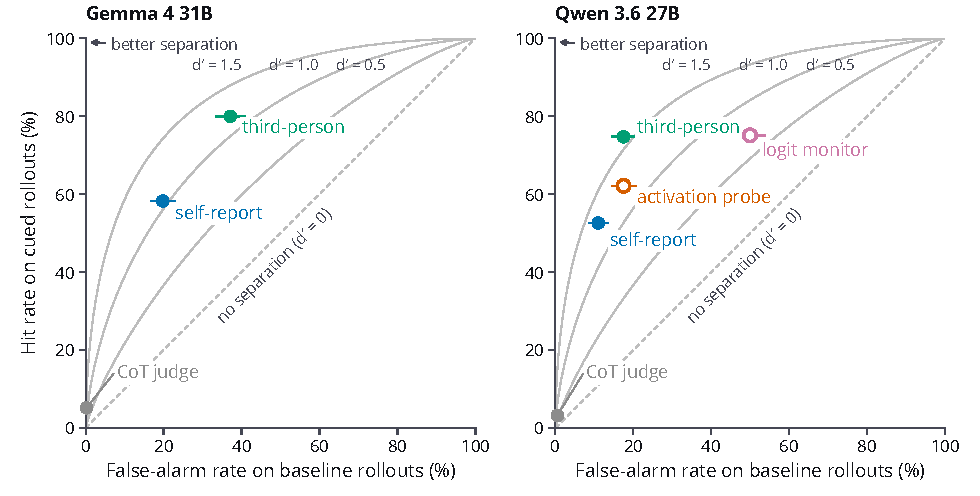
\includegraphics[width=\textwidth]{figures/fig1.pdf}
  \caption{\textbf{Every analysed detector flags cued rollouts more often. The CoT judge flags at most
  \cv{gemma/cot/hit}\% of cued rollouts, and every other detector more than half.}
  95\% exact intervals. Grey curves: equal $d'$ ($0.5$, $1.0$, $1.5$), the measure of how well a detector separates cued from baseline rollouts (Section~\ref{sec:method}).
  Open markers: white-box detectors, thresholds learned out of fold.}
  \label{fig:sensitivity}
\end{figure}

Because the benchmark adds the cues itself, we know which prompts carry them but not whether the
model noticed them. For this reason, we score detectors against the cue label as a proxy for
awareness. A detector's positive rate is the share of rollouts it flags. Its hit rate $H$ is its
positive rate on cued rollouts, and its false-alarm rate $F$ is its positive rate on baseline
rollouts. The detector separates the two groups if $H > F$, and we measure the separation with
$d' = \Phi^{-1}(H) - \Phi^{-1}(F)$, where $\Phi^{-1}$ maps a rate to a \mbox{$z$-score}. This
$d'$ is zero for a detector that ignores the cues. Under the equal-variance model, it is also
independent of the threshold (Figure~\ref{fig:sensitivity}; interval methods in
Appendix~\ref{app:formulas}).

The white-box detectors need the model's internal values. To get them, we fed each saved rollout
back through the model as input and recorded its activations and next-token probabilities
(teacher forcing). The probe reads only the prompt, so all repetitions of a prompt share one
prediction, whereas the logit monitor gives one prediction per rollout. Their thresholds and the
probe's layer were tuned on the cue labels by cross-validation grouped by task, so every
prediction is out of fold (Appendix~\ref{app:whitebox}).

On Gemma, however, the forward pass gave non-finite activations on \cv{gemma/reencode/nan} of
\cv{gemma/rollouts} rollouts, and the logit monitor failed on \cv{gemma/logit/nan}. The
non-finite activations were more common in long rollouts and in a few tasks, for reasons we
could not identify. Consequently, the usable rollouts are a non-random subset that could bias estimates,
so we exclude Gemma's white-box detectors (Appendix~\ref{app:gemma}).

We measure agreement with Cohen's $\kappa$ on the analysed rollouts, which are the baseline and
cued rollouts with a usable prediction. A rule fixed before the full run excludes any detector that
flags under \cv{run/floor}\% of these rollouts, because $\kappa$ is unreliable at such low rates.
Two detectors with different positive rates cannot agree perfectly. Their $\kappa$ reaches its
maximum $\kappa_{\max}$ when every positive of the rarer detector is also a positive of the other
(\citealp{feinstein1990high,byrt1993bias,cohen1960coefficient}; Appendix~\ref{app:formulas}).
The gap $1 - \kappa$ therefore has two parts. The first, $1 - \kappa_{\max}$, is forced by the
unequal rates. The second, $\kappa_{\max} - \kappa$, is the remaining disagreement, which comes from
flagging different rollouts and from a detector's inconsistency across repetitions. Because
$\kappa_{\max}$ differs by pair, we report $\kappa$ as a percentage of it
(Appendix~\ref{app:formulas}). A percentage at or below zero means no agreement beyond chance.

To remove the agreement that the cues alone create (Appendix~\ref{app:overall}), we use the
stratified $\kappa$. First, within each cue condition, we take the observed agreement and the
agreement expected by chance from that condition's positive rates. Then we sum both over the
conditions, weighting each condition by its number of rollouts, and form $\kappa$ from the two
sums (Appendix~\ref{app:formulas}). As a result, a shared response to the cues counts as chance
agreement. Similarly, the $\kappa_{\max}$ of the stratified $\kappa$ comes from the positive
rates within each condition. Our planned analysis used $d'$ and the $\kappa$ over all analysed
rollouts, so the stratified $\kappa$ and every comparison with $\kappa_{\max}$ are post hoc.
